\documentclass[10pt,a4paper]{article}
\usepackage[utf8x]{inputenc}
\usepackage[T1]{fontenc}
%\usepackage{stringenc} % for grffile
\usepackage{ucs}
\usepackage{amsthm} %numéroter les questions
\usepackage[english]{babel}
\usepackage{datetime}
\usepackage{xspace} % typographie IN
\usepackage{hyperref}% hyperliens
\usepackage[all]{hypcap} %lien pointe en haut des figures
\usepackage[english]{varioref} %voir x p y
\usepackage{fancyhdr}% en têtes
%\input cyracc.def
\usepackage[]{graphicx} %include pictures
%\usepackage[encoding,inputencoding=utf8,filenameencoding=utf8]{grffile}
%\usepackage[extendedchars,inputencoding=latin1,filenameencoding=latin1]{grffile}
\usepackage[siunitx ]{circuitikz}
\usepackage{gnuplottex}
\usepackage{ifthen}
\graphicspath{{./figures/}}
%\usepackage{array}
\usepackage{amsmath}
\usepackage[]{xcolor}
\usepackage{tikz}
\usepackage{tikz-timing}
\usetikzlibrary{scopes}
\usetikzlibrary{backgrounds}
\usepackage{listings}
\usepackage{enumitem}
\usepackage[top=1 in, bottom=1 in, left=1.3 in, right=1 in]{geometry} % Yeah, that's bad to play with margins
\usepackage[]{pdfpages}
\usepackage{pdflscape}
\usepackage[]{attachfile}
%\usepackage{colortbl}
%\usepackage{multirow}
\usepackage{booktabs}
\usepackage{makecell}
\usepackage[ ]{subfig}
%\usepackage{rotating}
\usepackage{upgreek}

\newdateformat{mydate}{2019--2020}%hack pour remplacer \THEYEAR

%cyr
%\newcommand\textcyr[1]{{\fontencoding{OT2}\fontfamily{wncyr}\selectfont #1}}


\newboolean{corrige}
%\setboolean{corrige}{true}%corrigé
\setboolean{corrige}{false}% pas de corrigé

\newboolean{annexes}
%\setboolean{annexes}{true}%annexes
\setboolean{annexes}{false}% pas de annexes

\newboolean{mos}
%\setboolean{mos}{true}%annexes
\setboolean{mos}{false}% pas de annexes

\usepackage{aeguill} %guillemets

%% fancy header & foot
\pagestyle{fancy}
\lhead{[ELEC-H-410] Real-Time systems Labo n° 2: \rtos}
\rhead{\mydate\today\\ page \thepage}
\chead{\ifthenelse{\boolean{corrige}}{Corrigé}{}}
\cfoot{}
%%

\pdfinfo{
    /Author (ULB -- BEAMS)
    /Title (Labo n° 2 ELEC-H-410)
    /ModDate (D:\pdfdate)
}

\hypersetup{
    pdftitle={Labo n° 2 [ELEC-H-410] Real-Time systems},
    pdfauthor={©2014-17 ULB - BEAMS},
    pdfsubject={FreeRTOS}
}

\theoremstyle{definition}% questions pas en italique
\newtheorem{E}{\color{blue}Exercise}[] % numéroter les questions [section] ou non []

\newcommand{\reponse}[1]{% pour intégrer une réponse : \reponse{texte} : sera inclus si \boolean{corrige}
	\ifthenelse {\boolean{corrige}} {\paragraph{Réponse :} #1} {}
 }

\newcommand{\addcontentslinenono}[4]{\addtocontents{#1}{\protect\contentsline{#2}{#3}{#4}{}}}

\newcommand{\on}[1]{\operatorname{#1}}

\newcommand{\reg}[1]{\texttt{reg#1}}

\newcommand{\rtos}{FreeRTOS}

\newcommand{\kw}[1]{\texttt{#1}}

\setlength{\parskip}{1ex plus .5ex minus .5ex} % espacement entre paragraphes
\setlength{\parindent}{0 ex plus 0ex minus 0 ex} % retrait en début de §

\def\labelitemi{--}
\setlist{parsep=0pt,itemsep=0pt,style=standard,leftmargin=\parindent, align=left} % pas d'espace prohibitif entre les items
\setlist{nolistsep}

\newcolumntype{C}[1]{>{\centering\let\newline\\\arraybackslash\hspace{0pt}}m{#1}}

%\setlength{\tabcolsep}{0pt} %no extra space in cells to keep constant tabular width

\date{\vspace{-1cm}\mydate\today}
\title{\vspace{-2cm} Labo n° 2\\ Real-Time systems [ELEC-H-410]\\ Sharing resources under \rtos~\ifthenelse{\boolean{corrige}}{~\\Corrigé}{}}

%\author{\vspace{-1cm}}%\textsc{Yannick Allard}}


\lstdefinestyle{customasm}{
	% belowcaptionskip=1\baselineskip,
	% frame=L,
	% xleftmargin=\parindent,
	language=[x86masm]Assembler,
	basicstyle=\footnotesize\ttfamily,
	commentstyle=\itshape\color{purple!40!black},
	comment=[l]//,
}
\lstdefinestyle{customc}{
    belowcaptionskip=1\baselineskip,
    breaklines=true,
    frame=L,
    xleftmargin=\parindent,
    language=C,
    showstringspaces=false,
    basicstyle=\footnotesize\ttfamily,
    keywordstyle=\bfseries\color{green!40!black},
    commentstyle=\itshape\color{purple!40!black},
    identifierstyle=\color{blue},
    stringstyle=\color{orange},
}
\lstset{escapechar=@,style=customc}

\begin{document}

	% Introduce a new counter for counting the nodes needed for circling
	\newcounter{nodecount}
	% Command for making a new node and naming it according to the nodecount counter
	\newcommand\tabnode[1]{\addtocounter{nodecount}{1} \tikz \node (\arabic{nodecount}) {#1};}

	% Some options common to all the nodes and paths
	\tikzstyle{every picture}+=[remember picture,baseline]
	\tikzstyle{every node}+=[inner sep=0pt,anchor=base]
	\tikzstyle{every path}+=[thick, rounded corners]

	% for tikz pict


	\maketitle
	In order  for you to work remotely, we changed this year project into a game. The game simulates a pandemic situation, very much like the one we are seeing right now. As you have seen, real-time response is a critical component of handling a pandemic efficiently. 

It is by no means our intention to take the current epidemic lightly. However, we thought that this project assignment would allow to lighten the mood a little, as everyone's morale will also be taking a serious hit during this period of confinement. Keep your spirits high and make sure you give your courses your best (all of them, not just this one). We will need talented and bright engineers in the aftermath of this crisis.  

To play this game, you don't need any equipment other than the PSOC itself.
The game is entirely coded inside one FreeRTOS task (\textit{gameTask}).
It sends "events" and we ask you to make a code that will automatically respond to those "events".\\
Depending on your response time you will increase or not some variables.

\subsection*{Useful documentation:}
\begin{itemize}
    \item Official \rtos~ documentation: \url{https://www.freertos.org/Documentation/RTOS_book.html}
    \item Getting Started with PSoC 5LP: \url{https://www.cypress.com/file/41436/download}
    \item Video example on how to use the PSoC: \url{https://www.cypress.com/video-library/PSoC}
    \item The extension board schematics: \texttt{Extension\_PSoC.pdf}
		\item Getting started with the Logic Analyzer: \url{https://learn.sparkfun.com/tutorials/using-the-usb-logic-analyzer-with-sigrok-pulseview}
\end{itemize}


	\section{Sharing resources}

The simplest way to make two tasks communicate is to use structures of shared data: most of the time they are global variables. It is then necessary to establish a mechanism of protection to control the access to these variables.

Open the project \kw{resource\_sharing}.
\E{
	~\\\vspace*{-1.5Em}
	\begin{itemize}
		\item Analyse the code, knowing that each task is executed only \textbf{once} (\kw{vTaskSuspend()} is called at the end of the \textit{for} loop), what should be the value of the global variable \kw{cntr} at the end of the execution?
		\item Compile and execute the code.
		\item Using a watch window and the debugger, check the value of \kw{cntr}. Is this the expected result? Why? (Use the logic analyser to help)
	\end{itemize}
}{}\reponse{
    \kw{cntr} should be $ 2 $ at the end of the execution.
    Go in debug mode, select Debug > Windows > Watch > 1 and type cntr.
    \kw{cntr} is equals to $ 1 $. 
}

%To protect the shared variables, uC/OS-II proposes two main solutions: \textbf{masking the interruptions} or using a \textbf{mutex}.

%The first solution is very efficient, but can only be used for very short lapses of time (shorter than the critical sections created by the RTOS itself), otherwise the latency time of the interruptions is increased and preemption of the task is blocked, which is against real-time.

The \textbf{mutex} (see chapter over priority-driven systems) is a convenient way to protect shared data, while still handling interrupts and authorise the preemption of the running task. Note: when a task acquires a resource via \kw{xSemaphoreGive()}, it should not forget to release it via \kw{xSemaphoreTake()}. A pseudo code is given in Listing \ref{lst:listing 1}.

\vbox{
\begin{lstlisting}[caption={Mutex declaration/use}, label={lst:listing 1}]
    // [...]
    SemaphoreHandle_t myMutex; // declaration as global variable
    myMutex = xSemaphoreCreateMutex(); // creation

    void function() {
        // [...]
        xSemaphoreTake( myMutex, portMAX_DELAY );
        // operations on the shared resource ...
        xSemaphoreGive( myMutex );
        // [...]
    }
\end{lstlisting}
}


The first 2 lines of Listing \ref{lst:listing 1} create a mutex by:
\begin{itemize}
    \item declaring a handler with the type \kw{SemaphoreHandle\_t}. This declaration must be global, so that the mutex is visible from anywhere in the program.
    \item creating the mutex.
\end{itemize}
For more details, see the official \rtos~ documentation.

\E{
    Modify the code of the \kw{ressource\_sharing} project by using a mutex to obtain the expected result for \kw{cntr}.
}{}


	\section{Deadlock problem}

Improper use of the mutex (or of any other mechanism of synchronisation between tasks) can bring
to a situation where no task can be executed anymore, this is called a \textit{deadlock} situation.

Open the \kw{Deadlock} project and launch its execution.

{Observe using the logic analyser that no task is executed although the tasks should be periodic.}{}

\E{Find the reason of this deadlock by drawing a time graph of the different calls to the mutexes}{}


\E{
    Fix this problem using the parameter \kw{xTicksToWait} of \kw{xSemaphoreTake()}.
}{}

	
	\section{Priority inheritance}

Mutexes in \rtos~ uses a particular version of the priority inheritance. 
If a high priority task blocks while attempting to obtain a mutex that is currently held by a lower priority task, then the priority of the task holding the token is temporarily raised to that of the blocking task. This mechanism is designed to ensure the higher priority task is kept in the blocked state for the shortest time possible, and in so doing minimise the 'priority inversion' that has already occurred\footnote{for more details see \url{https://www.freertos.org/Real-time-embedded-RTOS-mutexes.html}}.

Open the project \kw{prio\_inheritance}.

\E{
    Observe the mechanism with the logic analyser.
}{}

	\section{Use of a semaphore}

The semaphores (in a flag version) allows a synchronisation between tasks or between an interrupt service routine (ISR) and a task.

In the Listing \ref{lst:listing 2}, \kw{Task1} immediately goes to the ``waiting" state until another \kw{Task2} has
reached a certain point of its execution, then \kw{Task1} resumes its execution.

\begin{lstlisting}[caption={Semaphore example}, label={lst:listing 2}]
    SemaphoreHandle_t startTask1;
    startTask1 = xSemaphoreCreateBinary();
    
    Task1(){
        for(;;){
            xSemaphoreTake( startTask1, portMAX_DELAY ); // Task 1 goes "waiting"
            // [...]
        }
    }
    
    Task2(){
        for(;;){
            xSemaphoreGive( startTask1 ); //Task1 goes to "ready"
            // [...]
        }
    }
\end{lstlisting}

% It should be noted that several ``flags" can be posted in the same semaphore (counting semaphore). Thus a task can require that an event occurs several times before resuming its execution. In the same way, several tasks can synchronise on the same event if this event posts several flags in the same semaphore (each task gets one of the flags).

% For more information, see \uCOSII~user's manual pp 92-97.

Open the project entitled \kw{synchronisation}.

This project consists in decoding a sound from a waveform and send it to the jack output of the extension board (connect your own headphones !).
It makes use of the Digital to Analogue (DAC) block embedded in the Analogue Block Array of the board.
You may observe its configuration in the \kw{TopDesign} tab.

The project contains two tasks:
\begin{itemize}
    \item \kw{decodeTask}, which decodes a sound by batches of 64 samples (long execution time). It uses the \kw{decodeSoundFrame()} function.
    \item \kw{dacTask} which reads the decoded samples and sends them at 1kHz to the DAC connected to the jack output of the extension board.
\end{itemize} 

To ensure continuous streaming of the sound, two buffers of samples are being used (\kw{buf1[]} and \kw{buf[2]}). 
When one is being decoded by the \kw{decodeTask} task, the other one is played with the \kw{dacTask}. 
Of course this only works if both tasks are synchronised.
A first semaphore was placed in this code so that the first samples are not sent to the DAC before they actually have been decoded.
If you run the code you will see that this does not work.

\E{
    Modify the code so that a new batch of decoded samples is not written in one of the two buffers before the previous batch has been completely send to the DAC.
    You may need to add another semaphore.
}{}
%\E{Use an additional semaphore so that a new batch of decoded samples is not written in one of the two buffers (\kw{buf0[]} or \kw{buf1[]}) by \kw{AppTaskSpeex} before the previous batch has been completely send to the loudspeaker by \kw{AppTaskDac}. }{}


	\section{Queues}

Until now, we saw that the use of global variables made it possible to exchange information between two tasks. This method however presents some disadvantages among which the fact that a task is not automatically informed of a change of the variable. It is thus necessary that the task checks it periodically (polling) or that it announces any change via a mutex or semaphore.

To make this exchange easier, \rtos~implements another protocol: \textbf{queues}.

A task or an ISR can deposit a message in a queues. In a similar way, one or more tasks can receive a message in this queue.

Note: when we speak about ``message" under \rtos, it actually acts as any kind of structure copied in a reserved memory. The type of structure must obviously be known by the transmitting task as well as the receiving task(s).

% \begin{center}
%     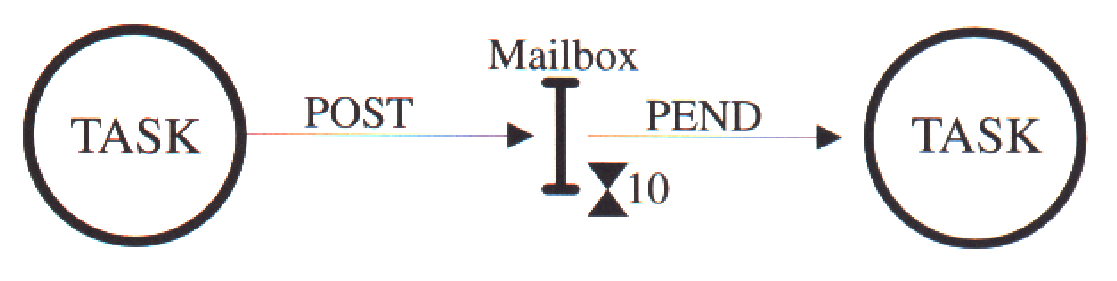
\includegraphics[width=12cm]{mailbox.png}
% \end{center}

If a task wishes to receive a message coming from a queue, it is suspended until the arrival of the message, or during a lapse of time defined by the application. Each queues is thus associated to a waiting list containing these suspended tasks. When the message is posted, it's the highest priority waiting task that receives the message\footnote{for more details see
\url{https://www.freertos.org/Embedded-RTOS-Queues.html}}.

Open the project \kw{keyboard}.
 
This project contains two tasks :
\begin{itemize}
    \item \kw{keyboardTask} is the task which manages the keyboard: if a new key is pressed, the \kw{key} variable contains the ASCII code of this key. The task is reactivated every 50ms to detect the actions of the user. It makes use of the \kw{KB\_Scan()} API of the block \kw{keyboard\_4x3}. This block was custom made for these labs and is part of the \kw{extensionBoardLib} library. Make sure your project includes the library by right clicking on the project tab > Dependencies and verify that the extensionBoardLib is checked. Also, make sure that the keyboard is correctly connected to the extension board, see Appendix~\ref{ap:kb}.
    \item \kw{lcdTask} displays a character on the LCD screen. Read the datasheet of the \kw{Character LCD} block to understand how it interact with the LCD screen.
\end{itemize}

\E{
    Create a queue allowing to transmit the characters pressed on the keyboard to the task displaying the characters on the screen. The queue should only contain one message.
}{}
%\marginpar{OK add caption and refr to listing} done


	
    \vfill
    \footnotesize{
        Found an error? Let us know: \url{https://github.com/BEAMS-EE/ELECH410/issues}
    }
    
    \newpage
    \appendix

\section{The \textit{Asix Sigma2} logic analyser}
\label{ap:la}

The Asix Sigma2 logic analyser is like:\\ 
\begin{center}
    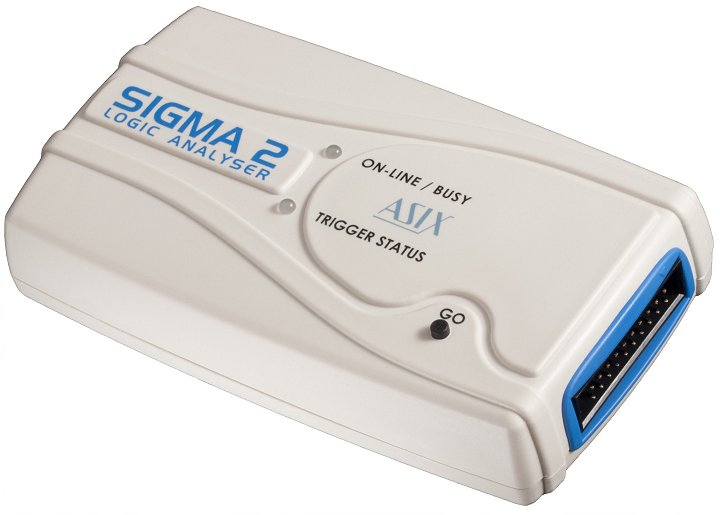
\includegraphics[width=4cm]{sigma2_720x515.jpg}
\end{center}

\subsection{Electrical connections to the Explorer 16 board}
    Connect the analyser to the extension board with the numbered ribbon cable following this scheme:
    \begin{center}
        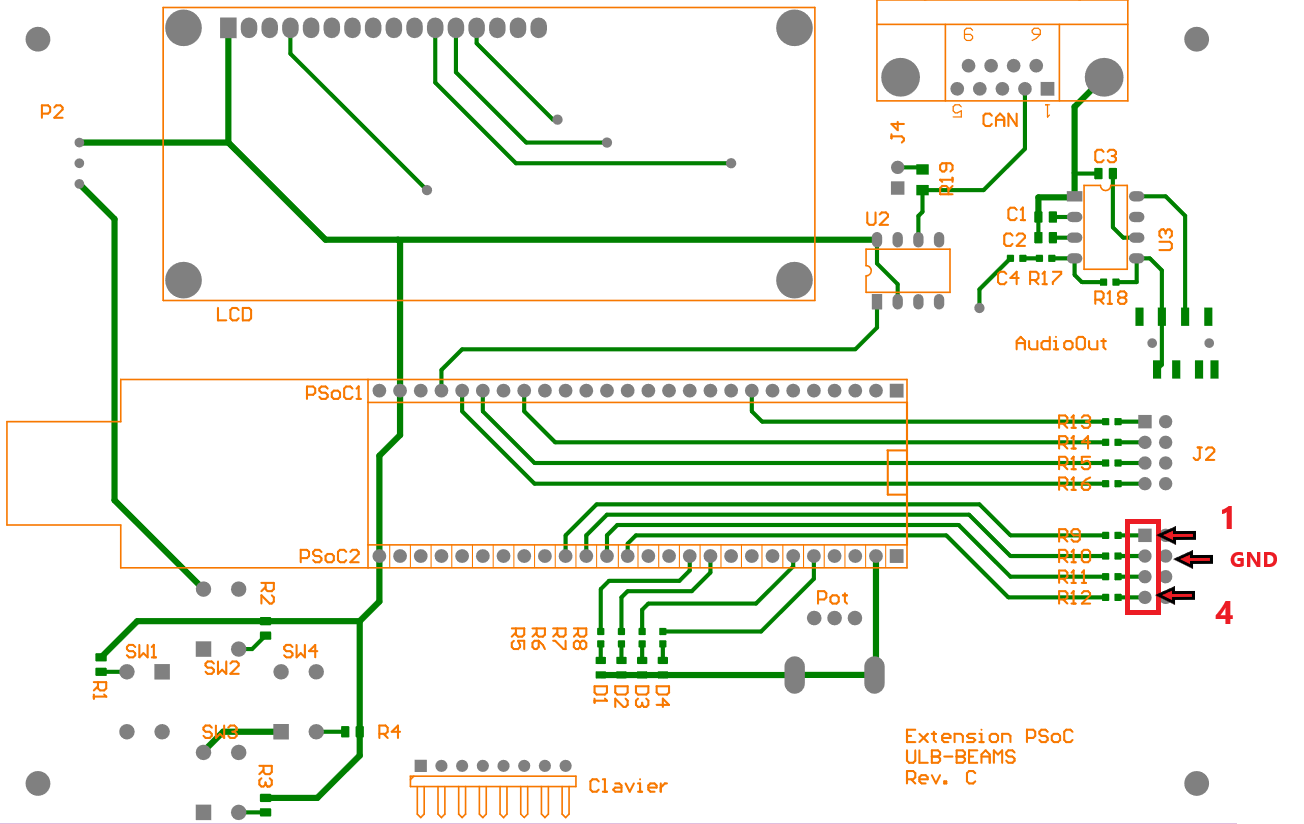
\includegraphics[width=0.7\textwidth]{analyserConnection.png}
    \end{center}

\subsection{Software on the computer}
    The software interface of the logic analyser looks like:
    \begin{center}
    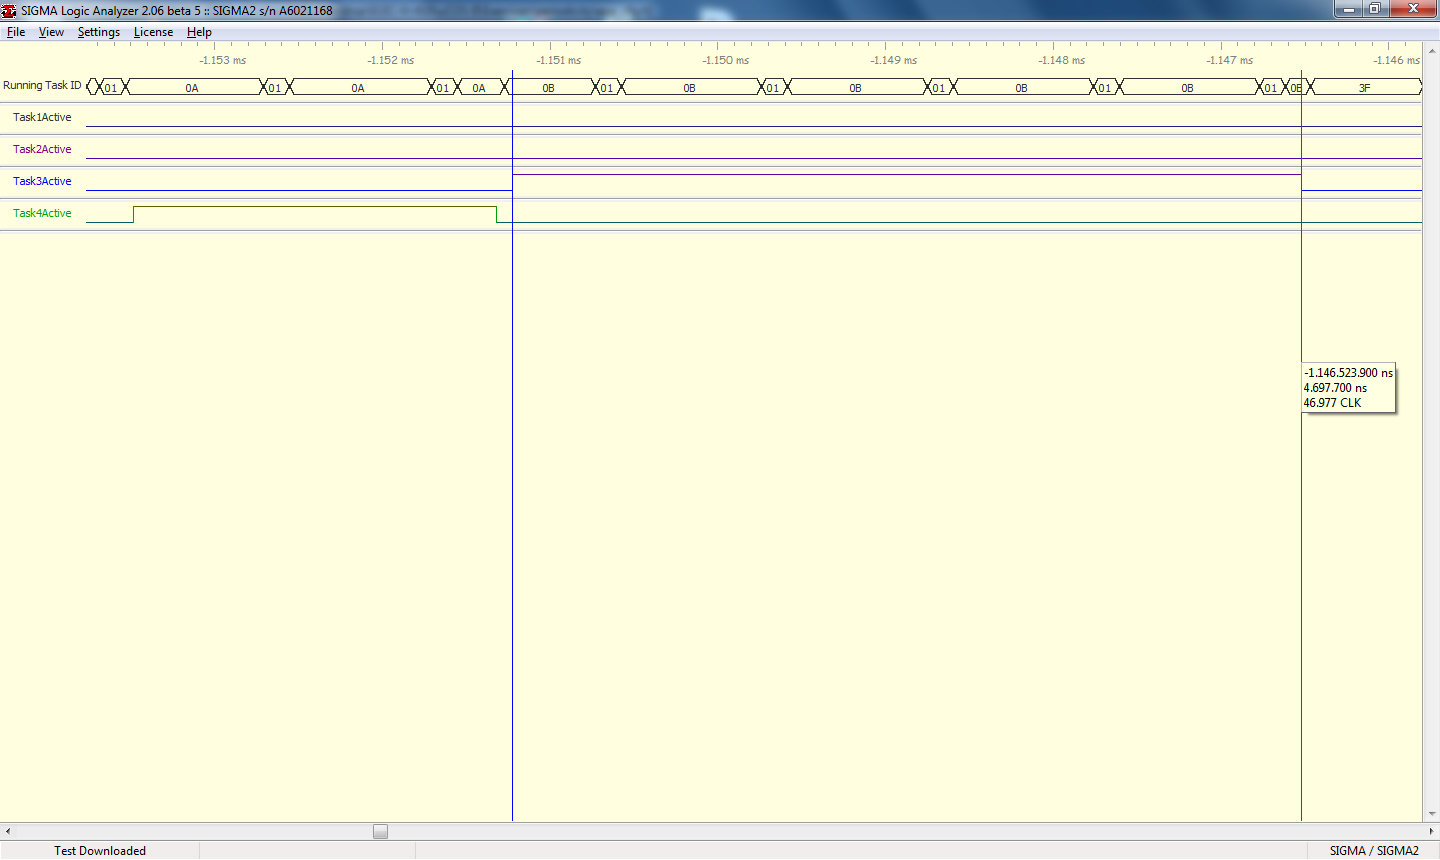
\includegraphics[width=13cm,trim= 0 100mm 0 0,clip]{Print_Screen_Logic_Analyzer.png}
    \end{center}

\subsection{Basic measurements}
    The red line on the screen is a cursor showing the time and values of signals in the main window. To place a marker (blue line), press space. If you move your cursor, the difference between the marker and the cursor will show in a tooltip.

    The first acquisition must be launched by software. Following acquisitions can be done using the ``go" button of the analyser.


\end{document}
